The work in \cite{mercer22} accomplishes a few things that are necessary background components for this work. First, it introduces a way of interpreting a CWP as a set of LTL properties and defines this method rigorously. Second, it introduces a method for translating a BPMN diagram into verifiable Promela code. Lastly, it uses a practical example in healthcare to show that the Promela and LTL can be used to verify the expected behavior of the original BPMN, represented as a CWP.

Our work expands on the work in \cite{mercer22}. A visual outline of our solution is shown in \figref{fig:NewSolutionRoadmap}. The original solution is colored blue with solid lines, while our additions are colored teal with dashed lines. 

In this section we give a summary of the work done in \cite{mercer22}. Their solution involves manually translating a CWP to a set of LTL properties and manually translating a BPMN to Promela code. Then, both inputs are given to a model checker, which outputs verification results for each LTL property. The solution works to verify a BPMN workflow, but there are some major downsides. Firstly, manual translation requires a lot of time and effort from a Promela expert. The translation process is also error-prone, even for an expert. Second, if the generated verification results indicate errors in the workflow, it is incredibly difficult to trace the counterexample back to the workflow to understand what is going wrong. 

Our additions aim to solve both of these problems, and they will be discussed later in \secref{sec:automatedGeneration} and \secref{sec:counterexample}.

\begin{figure*}[t]
  \begin{center}
    \begin{tabular}{c}
        \frame{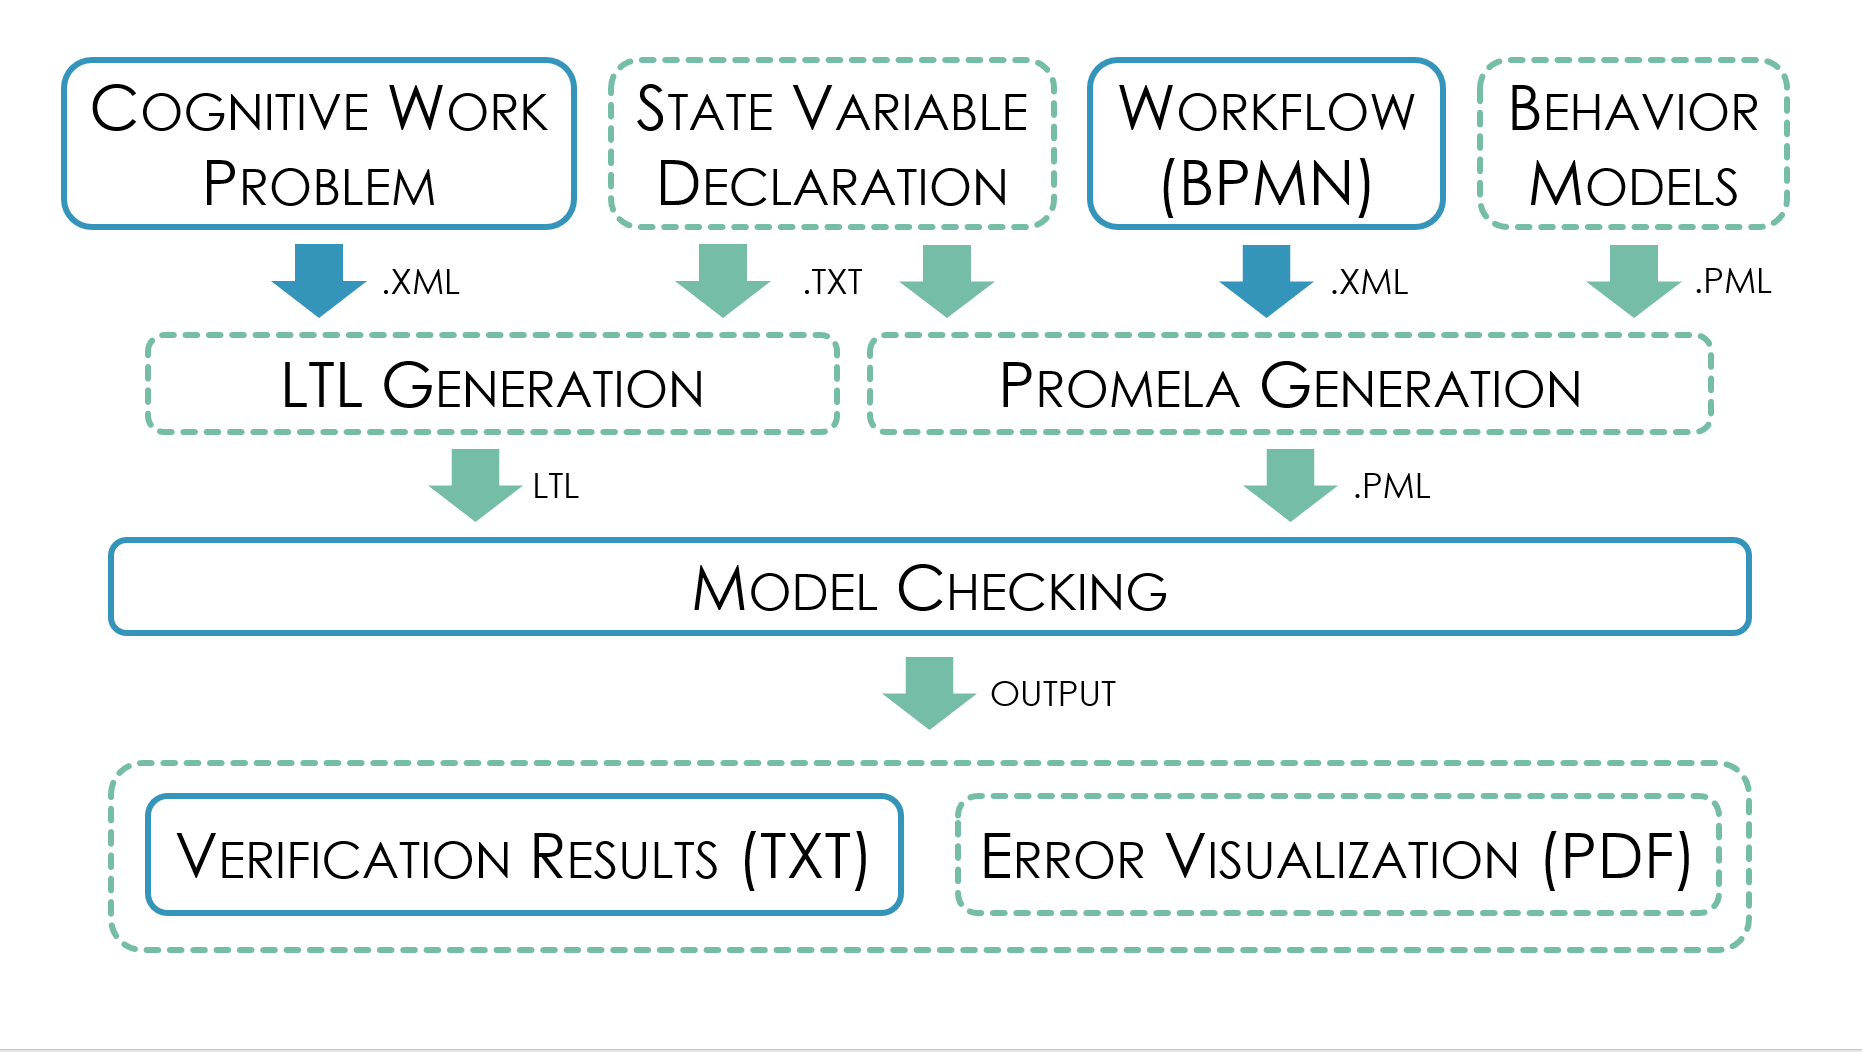
\includegraphics[width=\textwidth]{../figs/Other/NewSolutionDashedBoxes.png}}
    \end{tabular}
  \end{center}
\caption{Diagram of the automated BPMN verification solution. New elements are in Teal dashed boxes.}
\label{fig:NewSolutionRoadmap}
\end{figure*}
